\subsection{Mock-up dell'applicazione}
    \begin{flushleft}
        Qui vengono presentati i mockup relativi all'applicazione.
    \end{flushleft}
    \subsubsection{Homepage dell'applicazione}
        \begin{figure}[H]
            \centering
            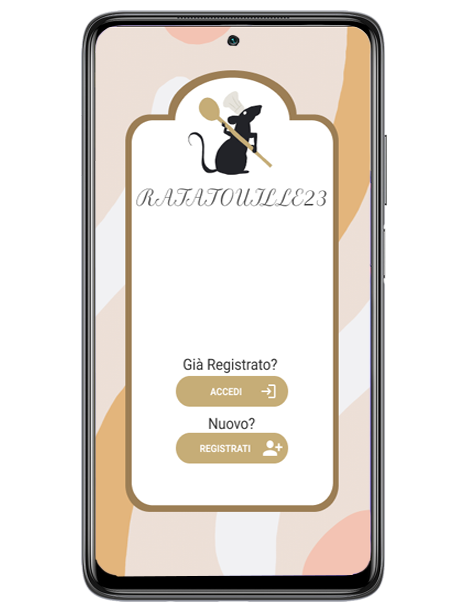
\includegraphics[scale=2.5]{assets/Mockup/Mockup_Homepage.png}
            \caption{\textbf{M01}: Homepage dell'applicazione}
            \label{fig:Mockup_Homepage}
        \end{figure}
        \begin{flushleft}
            \textbf{ID} \ \Large{\textit{\textbf{M01}}}\\
        \end{flushleft}

        \textbf{Componenti}:

        \begin{center}
          \begin{tblr}{hlines = {0.9pt}, vlines = {0.9pt}, row{1} = {pink!60}, colspec = {X[c]X[c]X[c]}, width = \textwidth}
            \textbf{Tipo}  &   \textbf{Nome} & \textbf{Funzione} \\
            Bottone        &   ACCEDI        & Quando cliccato porta alla schermata \textit{\textbf{M02}} \\
            Bottone        &    REGISTRATI   & Quando cliccato porta alla schermata \textit{\textbf{M03}} \\
          \end{tblr}
        \end{center}
        
        \newpage
        \subsubsection{Schermata di accesso nel sistema}
            \begin{figure}[H]
                \centering
                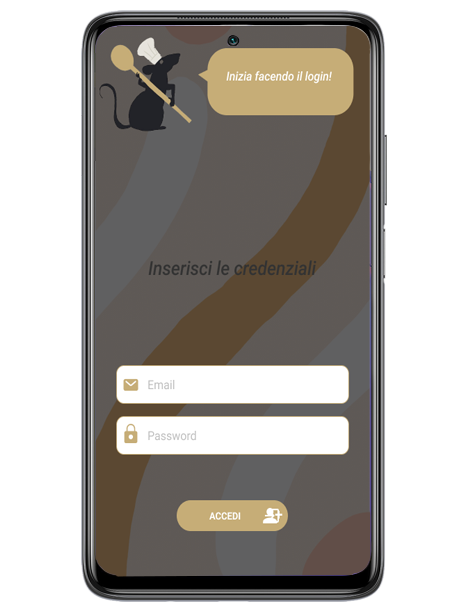
\includegraphics[scale=2.5]{assets/Mockup/Mockup_Accesso.png}
                \caption{\textbf{M02}: Schermata di accesso nel sistema}
                \label{fig:Mockup_Login}
            \end{figure}
            \begin{flushleft}
                \textbf{ID} \ \Large{\textit{\textbf{M02}}}\\
            \end{flushleft}

            \textbf{Componenti}:

            \begin{center}
              \begin{tblr}{hlines = {0.9pt}, vlines = {0.9pt}, row{1} = {pink!60}, colspec = {X[c]X[c]X[c]}, width = \textwidth}
                \textbf{Tipo}   &   \textbf{Nome}   &   \textbf{Funzione} \\
                Edit Text       &   EMAIL &   Permette l'inserimento dell'email dell'utente \\
                Edit Text & PASSWORD  &  Permette l'inserimento della password dell'utente  \\
                Bottone &   ENTRA   & Quando cliccato porta alla schermata \textit{\textbf{M04}} se admin, \textit{\textbf{M0?}} se dipendente \\
              \end{tblr}
            \end{center}

        \newpage
        \subsubsection{Schermata di registrazione nel sistema}
        \begin{figure}[H]
          \centering
          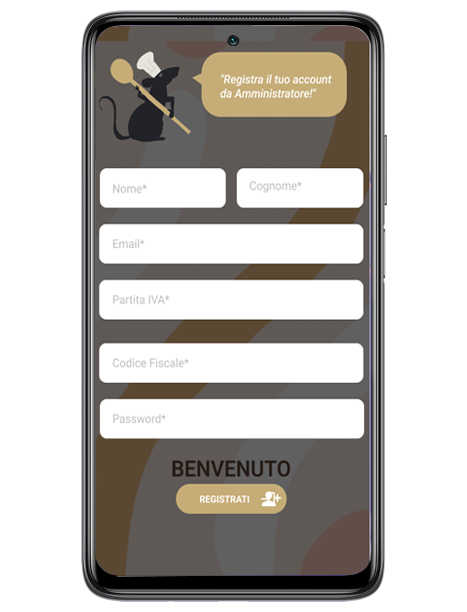
\includegraphics[scale=1.5]{assets/Mockup/Mockup_Registrazione.png}
          \caption{\textbf{M03}: Schermata di registrazione nel sistema}
          \label{fig:Mockup_Register}
        \end{figure}

        \begin{flushleft}
          \textbf{ID} \ \Large{\textit{\textbf{M03}}}\\
          \large{\textit{Nota}: la schermata di registrazione è valida solo per gli admin proprietari dei ristoranti, in quanto sono poi loro a registrare i dipendenti.}\\
        \end{flushleft}

        \textbf{Componenti}:

            \begin{center}
              \begin{tblr}{hlines = {0.9pt}, vlines = {0.9pt}, row{1} = {pink!60}, colspec = {X[c]X[c]X[c]}, width = \textwidth}
                \textbf{Tipo}   &   \textbf{Nome}   &   \textbf{Funzione} \\
                Edit Text    &   NOME    &   Permette di inserire il nome dell'admin \\
                Edit Text & COGNOME   &  Permette di inserire il cognome dell'admin \\
                Edit Text    &   PASSWORD    &   Permette di inserire una password per l'admin \\
                Edit Text    &   EMAIL   &   Permette di inserire l'email dell'admin \\
                Edit Text    & CODICE FISCALE    & Permette di inserire il codice fiscale dell'admin \\
                Edit Text    &   P.IVA   & Permette di inserire la partita IVA dell'admin \\
                Bottone &   REGISTRATI  & Quando cliccato riporta alla schermata \textit{\textbf{M01}} per permettere l'accesso \\
              \end{tblr}
            \end{center}
        \newpage
        \subsubsection{Schermata home per gli admin}
        \begin{figure}[H]
            \centering
            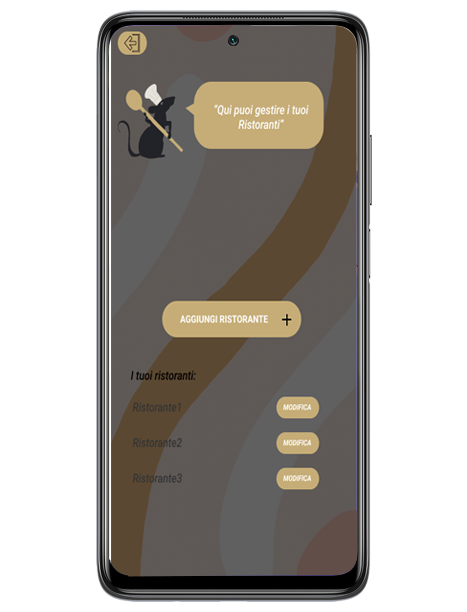
\includegraphics[scale=2.5]{assets/Mockup/Mockup_AdminDashboard.png}
            \caption{\textbf{M04}: Schermata home per gli admin}
            \label{fig:Mockup_AdminDashboard}
        \end{figure}
        \begin{flushleft}
            \textbf{ID} \ \Large{\textit{\textbf{M04}}} \\
        \end{flushleft}
        \textbf{Componenti}:

            \begin{center}
                \begin{tblr}{hlines = {0.9pt}, vlines = {0.9pt}, row{1} = {pink!60}, colspec = {X[c]X[c]X[c]}, width = \textwidth}
                \textbf{Tipo}   &   \textbf{Nome}   &   \textbf{Funzione} \\
                ScrollView &   I TUOI RISTORANTI    &   Visualizza ed eventualmente permette la modifica dei ristoranti registrati\\
                Bottone    &   AGGIUNGI RISTORANTE  &   Quando cliccato porta alla schermata \textit{\textbf{M05}} \\
                Bottone    &   MODIFICA   &   Quando cliccato porta alla schermata \textit{\textbf{M06}} \\
                \end{tblr}
            \end{center}
        \newpage

        \subsubsection{Schermata di registrazione di un nuovo ristorante}
        \begin{figure}[H]
            \centering
            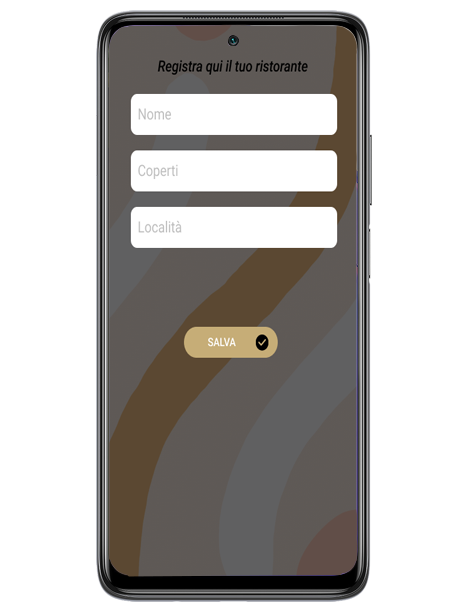
\includegraphics[scale=2]{assets/Mockup/Mockup_AddResturant.png}
            \caption{\textbf{M05}: Schermata di registrazione di un nuovo ristorante}
            \label{fig:Mockup_AddResturant}
        \end{figure}
        \begin{flushleft}
            \textbf{ID} \ \Large{\textit{\textbf{M05}}}
        \end{flushleft}
        \textbf{Componenti}:

        \begin{center}
          \begin{tblr}{hlines = {0.9pt}, vlines = {0.9pt}, row{1} = {pink!60}, colspec = {X[c]X[c]X[c]}, width = \textwidth}
            \textbf{Tipo}  &   \textbf{Nome}  & \textbf{Funzione} \\
            Edit Text      &   NOME           & Permette di inserire il nome del nuovo ristorante\\
            Edit Text      &   LOCALITA'      & Permette di inserire la località del nuovo ristorante\\
            Edit Text      &   COPERTI        & Permette di inserire il n° dei coperti del nuovo ristorante\\
            Bottone        &   SALVA          & Quando cliccato salva il nuovo ristorante nel database e torna alla schermata \textit{\textbf{M04}} \\
          \end{tblr}
        \end{center}
        \newpage
        \subsubsection{Schermata di modifica di un ristorante}
        \begin{figure}[H]
            \centering
            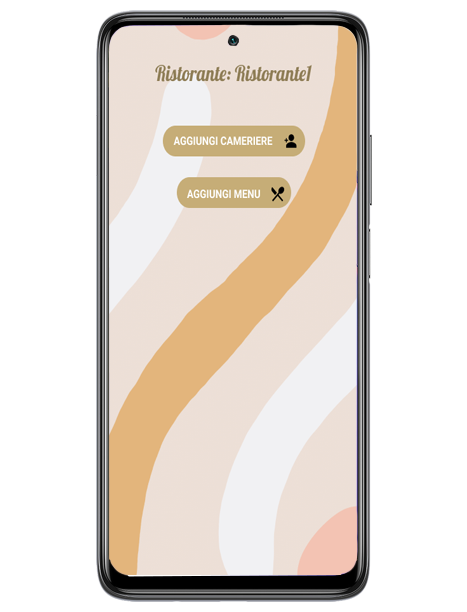
\includegraphics[scale=2.5]{assets/Mockup/Mockup_ResturantManager.png}
            \caption{\textbf{M06}: Schermata di modifica di un ristorante}
            \label{fig:Mockup_ResturantManager}
        \end{figure}
        \begin{flushleft}
            \textbf{ID} \ \Large{\textit{\textbf{M06}}}
        \end{flushleft}

        \textbf{Componenti}:

          \begin{center}
            \begin{tblr}{hlines = {0.9pt}, vlines = {0.9pt}, row{1} = {pink!60}, colspec = {X[c]X[c]X[c]}, width = \textwidth}
              \textbf{Tipo}  &   \textbf{Nome}  & \textbf{Funzione} \\
              \textbf{Tipo}   &   \textbf{Nome}   &   \textbf{Funzione} \\
              Bottone   &   AGGIUNGI CAMERIERE &   Quando cliccato porta alla schermata \textit{\textbf{M07}}\\
              Bottone   &   AGGIUNGI MENU &   Quando cliccato porta alla schermata \textit{\textbf{M08}}\\
            \end{tblr}
          \end{center}
        \newpage
        \subsubsection{Schermata di registrazione di un nuovo dipendente}
        \begin{figure}[H]
            \centering
            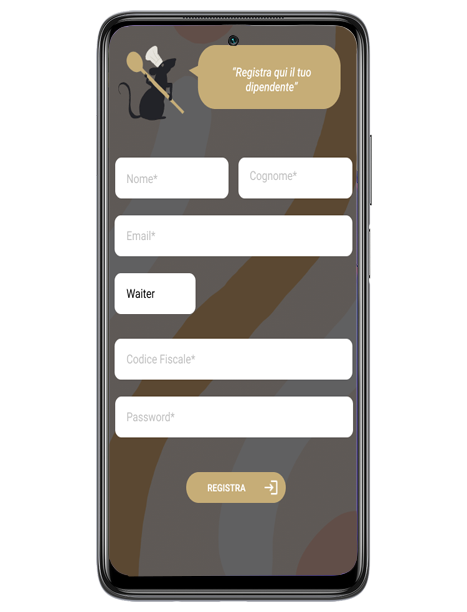
\includegraphics[scale=1.5]{assets/Mockup/Mockup_SaveWaiter.png}
            \caption{\textbf{M07}: Schermata di registrazione di un nuovo dipendente}
            \label{fig:Mockup_SaveWaiter}
        \end{figure}
        \begin{flushleft}
            \textbf{ID} \ \Large{\textit{\textbf{M07}}}
        \end{flushleft}
        \textbf{Componenti}:

        \begin{center}
          \begin{tblr}{hlines = {0.9pt}, vlines = {0.9pt}, row{1} = {pink!60}, colspec = {X[c]X[c]X[c]}, width = \textwidth}
            \textbf{Tipo}   &   \textbf{Nome}   &   \textbf{Funzione} \\
            Edit Text   &   NOME    &   Permette di inserire il nome del nuovo dipendente\\
            Edit Text   &   COGNOME   &   Permette di inserire il cognome del nuovo dipendente\\
            Edit Text   &   PASSWORD    &   Permette di inserire la password temporanea del nuovo dipendente  \\
            Edit Text   &   EMAIL   & Permette di inserire l'email del nuovo dipendente\\
            Edit Text   &   CODICE FISCALE    &   Permette di inserire il codice fiscale del nuovo dipendente \\
            Spinner &   {Waiter\\ (default)}    &   Permette di inserire il ruolo del nuovo dipendente \\
            Bottone &   REGISTRA    &   Quando cliccato, se tutti i dati sono corretti, riporta alla schermata \textit{\textbf{M04}} registrando il nuovo dipendente \\
          \end{tblr}
        \end{center}
        \newpage
        \subsubsection{Schermata di gestione del menù}
        \begin{figure}[H]
            \centering
            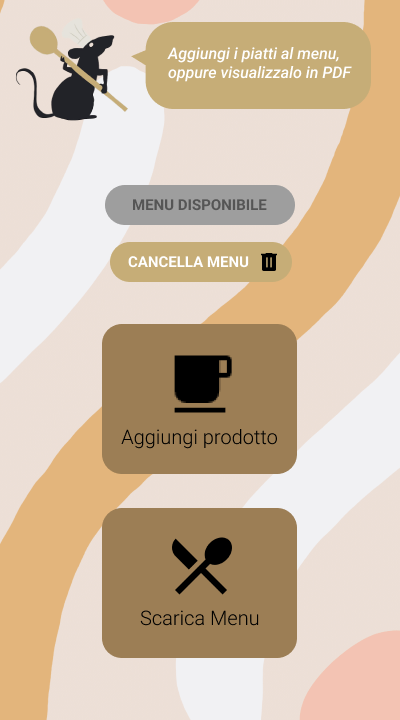
\includegraphics[scale=2.5]{assets/Mockup/Mockup_MenuManager.png}
            \caption{\textbf{M08}: Schermata di gestione del menù}
            \label{fig:Mockup_MenuManager}
        \end{figure}
        \begin{flushleft}
            \textbf{ID} \ \Large{\textit{\textbf{M08}}}
        \end{flushleft}
        \textbf{Componenti}:

        \begin{center}
          \begin{tblr}{hlines = {0.9pt}, vlines = {0.9pt}, row{1} = {pink!60}, colspec = {X[c]X[c]X[c]}, width = \textwidth}
            \textbf{Tipo}   &   \textbf{Nome}   &   \textbf{Funzione} \\
            Bottone   &   AGGIUNGI PRODOTTO    &   Quando cliccato porta alla schermata \textit{\textbf{M0?}}\\
            Edit Text   &   GENERA MENU   &   Permette di generare il menù e salvarlo sul dispositivo in formato PDF\\
          \end{tblr}
        \end{center}
